\subsection{Complex functions}

\subsubsection{Analytic functions}
\textbf{(a) Definitions}

\begin{itemize}
	\item \textbf{Complex functions}: A complex function $f$ is a function of the \verb|complex variable| $z=x+iy$ that results in a complex-valued output
	$$
	f(z) = u(x,y) + iv(x,y)
	$$
	where $u(x,y)$ and $v(x,y) $ are \verb|real| functions of \verb|two| variables.
	\item \textbf{Continuous}: A complex function is continuous at a point $z_0$ if and only if for any \verb|neighborhood| $\mathcal{V}$ of $f(z_0)$, $f^{-1}(\mathcal{V})$ is a neighborhood of $z_0$. 
	\begin{figure}
	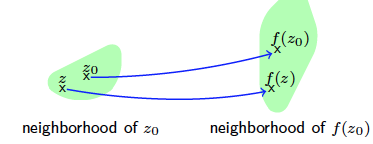
\includegraphics{figures/screenshot/screenshot.png}
	\end{figure}
\end{itemize}